\documentclass[10pt,a4paper]{article}
\usepackage[utf8x]{inputenc}
\usepackage{ucs}
\usepackage[left=2.00cm, right=2.00cm, top=2.00cm, bottom=2.00cm]{geometry}
\renewcommand\familydefault{\sfdefault}

\title{Summary - \lecture}
\author{}
\date{}


%costum layout
\setlength{\parindent}{0cm}
\usepackage{fancyhdr}
\pagestyle{fancy}
\fancyhf{}
\fancyhead[L]{
	\strut\rlap{\colorlayout\rule[-\dp\strutbox]{\headwidth}{\headheight}}
	\textcolor {white} {Summary: \lecture}}
\fancyfoot[L]{
	\strut\rlap{\colorlayout\rule[-\dp\strutbox]{\headwidth}{\headheight}}
	\textcolor {white} {last changed: \today}}
\fancyhead[R]{\textcolor{white}{\semseter}}
\fancyfoot[R]{\textcolor{white} {\thepage}}


%math
\usepackage{amsmath}
\usepackage{amsfonts}
\usepackage{amssymb}
\usepackage{amstext}
\usepackage{mathtools}


%graphics
\usepackage{graphicx}
\usepackage{floatflt}
\usepackage{float}


%tabular
\usepackage{tabularx}
\usepackage[font=small,labelfont=small]{caption}
\usepackage{colortbl}
\usepackage[dvipsnames]{xcolor}
\renewcommand{\arraystretch}{1}
%\arrayrulecolor{white}


%tikz
\usepackage{tikz}
\usetikzlibrary{shapes, petri}
\tikzstyle{ell}=[ellipse,draw, yshift=-2mm]
\tikzstyle{rec} = [rectangle, draw]
\tikzstyle{dia} = [diamond, aspect=2, draw, yshift=-5mm]
\tikzstyle{cir} = [circle, draw, minimum size=3mm]
\tikzstyle{arrHV} = [to path={-| (\tikztotarget)}]
\tikzstyle{arrVH} = [to path={|- (\tikztotarget)}]
\tikzstyle{whileright} = [xshift=20mm, yshift=-3mm]
\tikzstyle{whileleft} = [xshift=-20mm, yshift=-3mm]
\tikzstyle{txtright} = [above, xshift=15mm]
\tikzstyle{txtleft} = [above, xshift=-15mm]
\tikzstyle{empty} = [coordinate]
\usetikzlibrary{positioning}


%listings
\usepackage{listings}
\lstdefinestyle{costum} {
	language=Bash,
	basicstyle=\footnotesize\ttfamily,
	keywordstyle=\bfseries\color{cyan!50!blue},
	commentstyle=\itshape\color{black!50},
	%identifierstyle=\color{blue},
	stringstyle=\color{green!50!black},
	morekeywords={returns, loop, each},
	escapeinside={\%*}{*)}
}
\lstset{style=costum}


%custom title color
\usepackage{titlesec}
\setcounter{secnumdepth}{4}

\titleformat{\section}
{\color{cyan!80!blue}\normalfont\Large\bfseries}
{\color{cyan!80!blue}\thesection}{1em}{}

%\titleformat{\subsubsection}
%{\color{blue!30!black!70}\normalfont\bfseries}
%{\color{black}\thesection}{1em}{}
%
%\titleformat{\paragraph}
%{\color{green!30!black!70}\normalfont\normalsize\bfseries}{\theparagraph}{1em}{}
%\titlespacing*{\paragraph}
%{0pt}{3.25ex plus 1ex minus .2ex}{1.5ex plus .2ex}


%tab
\newcommand{\tab}[1][1]{\hspace*{#1cm}}


%hyperref
\usepackage{hyperref}


%vector
\newcommand{\vect}[1]{\ensuremath{\begin{bmatrix}#1\end{bmatrix}}}

\usepackage{pgfplots}

%TODO
%config
\newcommand{\lecture}{Introduction to Deep Learning} %title of the lecture
\newcommand{\lecturer}{Nießner M.} %lecturer of the lecture
\newcommand{\semseter}{summer semester 2020} %semester of this lecture, e.g., summer semester 2019
\newcommand{\colorlayout}{\color{cyan!50!blue}} %color of the title bar, see colors

%colors, e.g,
%cyan!50!blue
%green!50!black
%orange!50!black

%user
\newcommand{\cons}{\textcolor{red}{\textbf{-}}}
\newcommand{\pros}{\textcolor{green}{\textbf{+}}}


%TODO
% a user defined todo list



\begin{document}
\tableofcontents
\pagebreak

\section{Machine Learning Basics}
\subsection{Un-/Supervised Learning}
\begin{itemize}
	\item Unsupervised Learning
	\begin{itemize}
		\item No label or target class
		\item Find out properties of the structure of the data
		\item clustering (k-means, PCA, etc.)
	\end{itemize}
	\item Supervised Learning
	\begin{itemize}
		\item Labels or target classes
	\end{itemize}
	\item Reinforcement Learning
\end{itemize}

\subsection{Dataset}
\begin{itemize}
	\item Split dataset into
	\begin{itemize}
		\item Training data (e.g. 60\%) - Used to train the model
		\item Validation data (e.g. 20\%) - Validate the current model to find the best hyperparameters
		\item Test data (e.g. 20\%) - Is only used once in the end
	\end{itemize}
\end{itemize}

\pagebreak
\section{Linear Models}
\subsection{Regression, Classification}
\begin{itemize}
	\item \textbf{Regression:} Predicts a continuous output value
	\item \textbf{Classification:} Predicts a discrete value
	\begin{itemize}
		\item \textbf{Binary Classification:} Output either $0$ or $1$
		\item \textbf{Multi-class classification:} Set of N classes
	\end{itemize}
\end{itemize}

\subsection{Obtaining the model}
\begin{enumerate}
	\item Estimating using current model
	\item Calculating loss
	\item Optimizing the model
\end{enumerate}

\subsection{Linear Regression}
\subsubsection{Linear Model}
\begin{tabular}{ll}
	$i$: & index of current sample \\
	$j$: & index of current weight \\
	$d$: & input dimension/number of weights \\
	$x_{ij}$: & $i$-th input data/feature of the $j$-th weight \\
	$\theta_0$: & bias \\
	$\theta_j$: & weights \\
	$\hat y_i$: & $i$-th Prediction/Estimation (predicted label)
\end{tabular}

$$
	\hat y_i = \theta_0 + \sum_{j = 1}^d x_{ij} \theta_j = \theta_0 + x_{i1} \theta_1 + \dots + x_{id} \theta_d
$$

\textbf{Matrix Notation:}
$$
	\hat y = X \theta
$$

\subsubsection{Loss function}
Measures how good my estimation is and tells the optimization method how to make it better

\paragraph{Linear Least Squares:} ~\\
\begin{tabular}{ll}
	$n$: & number of training samples \\
	$y$: & Ground truth labels \\
	$\hat y$: & Estimated labels
\end{tabular}
$$
	J(\theta) = \frac 1 n \sum_{i = 1}^n (\hat y_i - y_i)^2
$$

\textbf{Matrix Notation:}
$$
	J(\theta) = (X \theta - y)^T (X \theta - y) = (\hat y - y)^T (\hat y - y)
$$

\subsubsection{Optimization}
Changes the model in order to improve the loss function/estimation
$$
	\theta = (X^TX)^{-1}X^Ty
$$

\subsection{Logistic Regression}
\subsubsection{Model}
\begin{tabular}{ll}
	$i$: & index of current sample \\
	$j$: & index of current weight \\
	$d$: & input dimension/number of weights \\
	$x_{ij}$: & $i$-th input data/feature of the $j$-th weight \\
	$\theta_j$: & model parameters \\
	$\hat y_i$: & $i$-th Prediction/Estimation (predicted label)
\end{tabular}

$$
	\hat y_i = \sigma(x_i \theta) = \sigma \left(\sum_{j = 1}^d x_{ij} \theta_j \right)
$$
with
$$
	\sigma(x) = \frac 1 {1 + e^{-x}}
$$

\subsubsection{Loss function}
Measures how good my estimation is and tells the optimization method how to make it better

\paragraph{Binary Cross-Entropy:} ~\\
\begin{tabular}{ll}
	$y$: & Ground truth labels \\
	$\hat y$: & Estimated labels
\end{tabular}
$$
	\mathcal L(\hat y_i, y_i) = y_i \log \hat y_i + (1 - y_i) \log (1 - \hat y_i)
$$

\subsubsection{Cost function}
\begin{tabular}{ll}
	$n$: & number of labels
\end{tabular}
$$
	C(\theta) = - \frac 1 n \sum_{i = 1}^n \mathcal L(\hat y_i, y_i)
$$

\subsubsection{Optimization}
Changes the model in order to improve the loss function/estimation
\begin{itemize}
	\item No closed-form solution
	\item Make use of an iterative method e.g. Gradient Descent
\end{itemize}

\section{Computational Graphs}
\begin{itemize}
	\item Directional graph
	\item Matrix operations are represented as compute graphs
	\item Vertex nodes are variables or operators like $+, -, *, /, log(), exp(), \dots$
	\item Directional edges show flow of inputs to vertices
	\item Neural network can be represented as computational graph
\end{itemize}

\subsection{Graphical representation}
\textbf{Example}
$$
	f(x, y, z) = (x + y) ⋅ z
$$
\begin{figure}[H]
	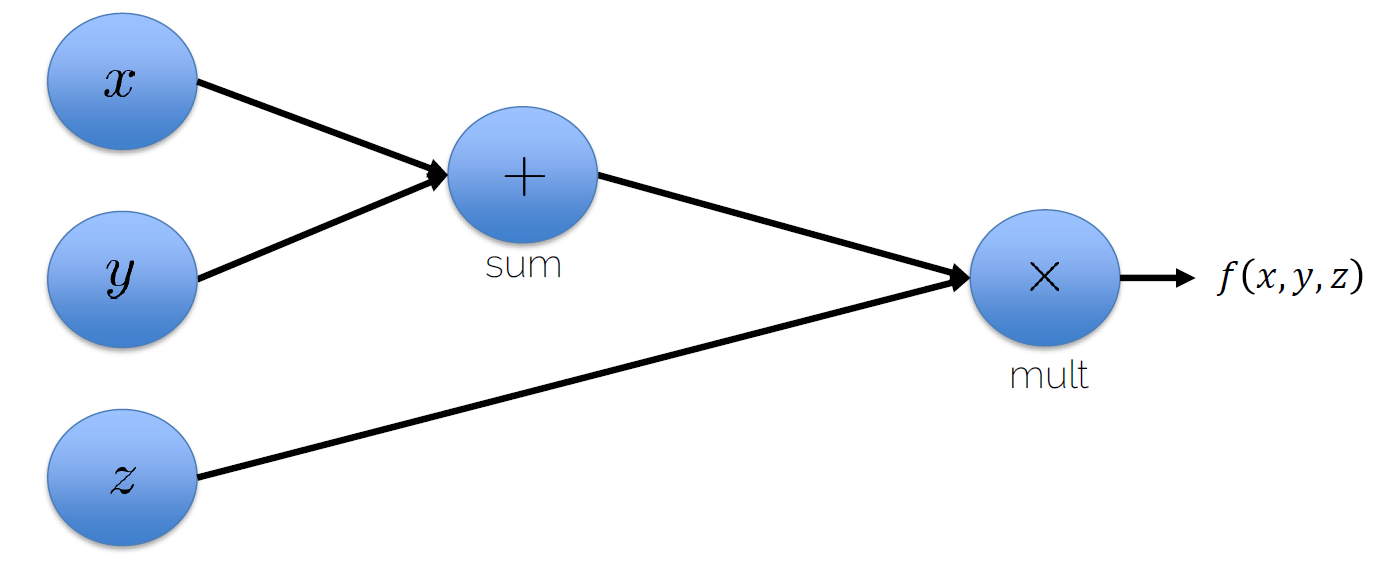
\includegraphics[width=\columnwidth]{figures/comp_graph.png}
\end{figure}

\textbf{Neural Network as Computational Graph}
\begin{figure}[H]
	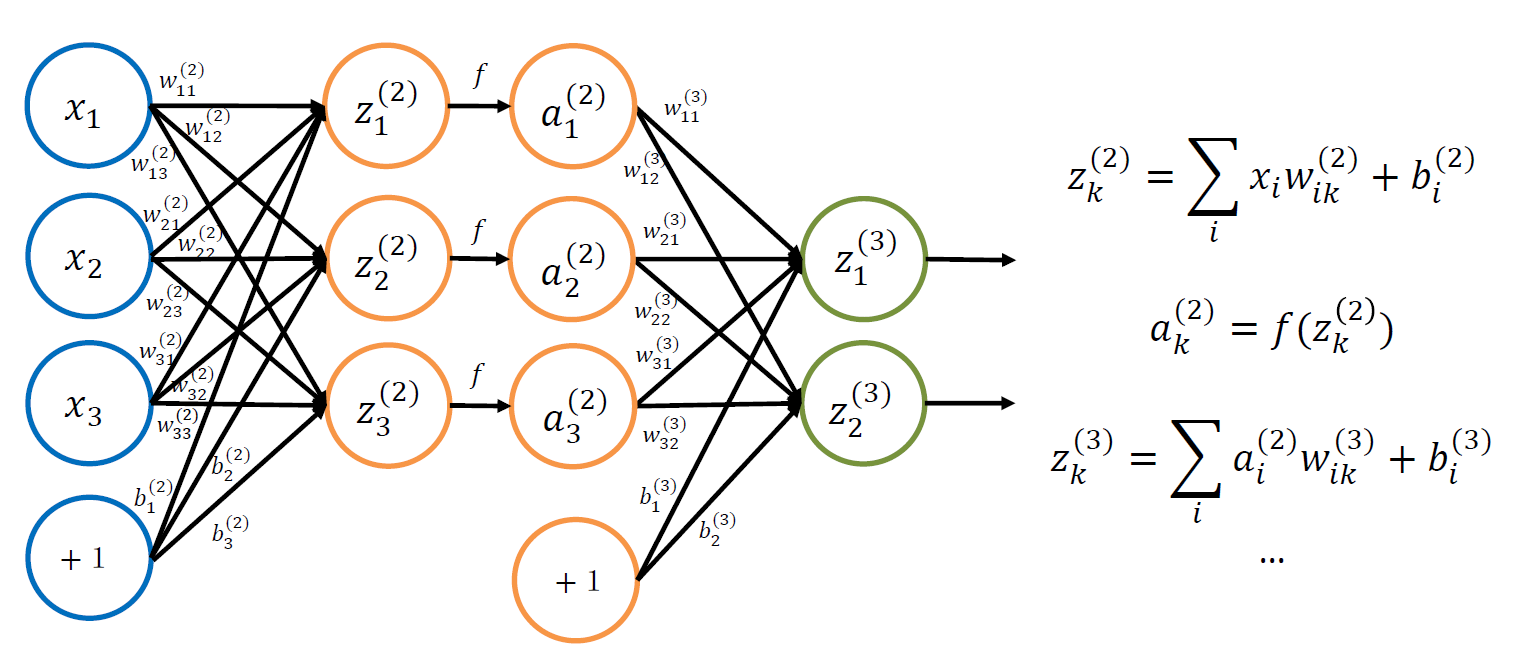
\includegraphics[width=\columnwidth]{figures/comp_graph_nn.png}
\end{figure}

\section{Neural Network}
\subsection{Activation Functions}
\subsubsection{Description}
%TODO

\subsubsection{Sigmoid}
\begin{tabularx}{\columnwidth}{XX}
	$$
	\sigma(x) = \frac 1 {1 + e^{-x}}
	$$ &\\&
	
	\begin{tikzpicture}
	\begin{axis}[
	xmin=-10, xmax=10,
	ymin=-0, ymax=1,
	axis y line=middle,
	axis x line=middle,
	]
	\addplot+[domain=-10:10, samples=100, mark=none] {1/(1 + exp(-x))};
	\end{axis}
	\end{tikzpicture}
\end{tabularx}


\subsubsection{Tanh(x)}
\begin{tabularx}{\columnwidth}{XX}	
	$$
	\tanh(x)
	$$ &\\&
	
	\begin{tikzpicture}
	\begin{axis}[
	xmin=-10, xmax=10,
	ymin=-1, ymax=1,
	axis y line=middle,
	axis x line=middle,
	]
	\addplot+[domain=-10:10, samples=100, mark=none] {tanh(x)};
	\end{axis}
	\end{tikzpicture}
\end{tabularx}

\subsubsection{ReLU}
\begin{tabularx}{\columnwidth}{XX}	
	$$
	\max(0, x)
	$$ &\\&
	
	\begin{tikzpicture}
	\begin{axis}[
	xmin=-10, xmax=10,
	ymin=0, ymax=10,
	axis y line=middle,
	axis x line=middle,
	]
	\addplot+[domain=-10:10, samples=100, mark=none] {max(0,x)};
	\end{axis}
	\end{tikzpicture}
\end{tabularx}

\subsubsection{Leaky ReLU}
\begin{tabularx}{\columnwidth}{XX}	
	$$
	\max(0.1x, x)
	$$ &\\&
	
	\begin{tikzpicture}
	\begin{axis}[
	xmin=-10, xmax=10,
	ymin=-1, ymax=10,
	axis y line=middle,
	axis x line=middle,
	]
	\addplot+[domain=-10:10, samples=100, mark=none] {max(0.1*x,x)};
	\end{axis}
	\end{tikzpicture}
\end{tabularx}

\subsubsection{Parametric ReLU}
$$
\max(\alpha x, x)
$$

\subsubsection{ELU}
$$
f(x) = \begin{cases}
x & \text{if } x > 0 \\
\alpha (e^x - 1) & \text{if } x ≤ 0
\end{cases}
$$

\subsubsection{Maxout}
$$
\max(w_1^Tx + b_1, w_2^T x + b_2)
$$



\subsection{Loss Function}
\subsubsection{Description}
A function to measure the goodness of the predictions
\begin{itemize}
	\item Large loss $\implies$ bad predictions
	\item Goal: Minimize the loss $\iff$ Find better predictions
	\item Choice of the loss function depends on the concrete problem or the distribution of the target variable
\end{itemize}

\subsubsection{Parameters}
\begin{tabular}{ll}
	$y$: & Ground truth \\
	$\hat y$: & Prediction \\
	$n$: & number of training samples \\
	$k$: & number of classes
\end{tabular}

\subsubsection{L1 Loss}
$$
	\mathcal L(y, \hat y; \theta) = \frac 1 n \sum_i^n ||y_i - \hat y_i||_1
$$

\subsubsection{MSE Loss}
$$
	\mathcal L(y, \hat y; \theta) = \frac 1 n \sum_i^n ||y_i - \hat y_i||_2^2
$$

\subsubsection{Binary Cross Entropy}
$$
	\mathcal L(y, \hat y; \theta) = - \sum_{i = 1}^n (y_i \log \hat y_i + (1 - y_i) \log(1 - \hat y_i))
$$

\subsubsection{Cross Entropy}
$$
	\mathcal L(y, \hat y; \theta) = - \sum_{i = 1}^n \sum_{j = 1}^k (y_{ij} \log \hat y_{ij})
$$

\subsection{Optimization Functions}
\subsubsection{General Optimization}
\begin{itemize}
	\item \textbf{Goal:} $\theta^* = \arg\min f(\theta, x, y)$
	\item \textbf{Linear Systems (Ax = b)}
	\begin{itemize}
		\item LU, QU, Cholesky, Jacobi, Gauss-Seidel, CG, PCG, ...
	\end{itemize}
	\item \textbf{Non-linear systems} (Gradient based methods):
	\begin{itemize}
		\item First order methods:
		\begin{itemize}
			\item Gradient Descent, SGD, SGD with Momemtum, RMSProp, Adam (Standard)
		\end{itemize}
		\item Second order methods (faster than first order methods, but only for full batch updates):
		\begin{itemize}
			\item Newton, Gauss-Newton, Levenberg-Marquardt, (L)BFGS
		\end{itemize}
	\end{itemize}
\end{itemize}


\subsubsection{Gradient Descent}
\begin{itemize}
	\item Finds local minimum
	\item Does not guarantee to find global optimum
	\item Does gradient steps in direction of negative gradient
	\item[\cons] Requires a lot of memory $\implies$ extremely expensive
\end{itemize}

Parameters: \\
\begin{tabular}{ll}
	$f(\theta, x_{1..n}, y_{1..n})$: & Function describing the neural network (including loss function) \\
	$x_{1..n}$: & Input vectors for all $n$ training samples \\
	$y_{1..n}$: & Ground truth for all $n$ training samples \\
	$\theta^k = \{W, b\}$: & Model Parameters at step $k$ \\
	$\alpha$: & Learning rate
\end{tabular} \\

Gradient Step:
$$
	\theta^{k + 1} = \theta^k - \alpha \nabla_\theta f(\theta^k, x_{1..n}, y_{1..n})
$$

\subsubsection{Stochastic Gradient Descent}
\begin{itemize}
	\item Split training set into several minibatches
	\item Minibatch size:
	\begin{itemize}
		\item Is a hyperparameter
		\item Is typically a power of 2
		\item Smaller batch size $\implies$ Greater variance in the gradients
		\item Is mostly limited by GPU memory
	\end{itemize}
	\item Epoch: Complete pass through training set
	\item[\cons] Cannot independently scale directions
	\item[\cons] Need to have conservative min learning rate to avoid divergence
	\item[\cons] Is slower than necessary
\end{itemize}

Parameters: \\
\begin{tabular}{ll}
	$n$: & Number of total training samples \\
	$m$: & Minibatch size (number of training samples per minibatch) \\
	$n/m$: & Number of minibatches \\
	$f(\theta, x_{1..m}, y_{1..m})$: & Function describing the neural network (including loss function) \\
	$x_{1..m}$: & Input vectors for one minibatch \\
	$y_{1..m}$: & Ground truth for one minibatch \\
	$\theta^k = \{W, b\}$: & Model Parameters at step $k$\\
	$k$: & iteration in current epoch \\
	$\alpha$: & Learning rate
\end{tabular} \\

Gradient Step:
$$
	\theta^{k + 1} = \theta^k - \alpha \nabla_\theta f(\theta^k, x_{1..m}, y_{1..m})
$$

\paragraph{Convergence of Stochastic Gradient Descent} ~\\
$f(\theta, x, y)$ converges to a local (global) minimum if:
\begin{enumerate}
	\item $\alpha_n ≥ 0, \forall n ≥ 0$
	\item $\sum_{n = 1}^∞ \alpha_n = ∞$
	\item $\sum_{n = 1}^∞ \alpha_n^2 < ∞$
	\item $f(\theta, x, y)$ ist strictly convex
\end{enumerate}
where $\alpha_1, \dots, \alpha_n$ is a sequence of positive step-sizes

\subsubsection{Gradient Descent with Momentum}
\begin{itemize}
	\item Step will be largest when a sequence of gradients all point to the same direction
\end{itemize}

Parameters: \\
\begin{tabular}{ll}
	$f(\theta, x, y)$: & Function describing the neural network (including loss function) \\
	$x$: & Input vectors \\
	$y$: & Ground truth \\
	$\theta^k = \{W, b\}$: & Model Parameters at step $k$\\
	$\alpha$: & Learning rate \\
	$\beta$: & Accumulation rate (friction, momentum), default: 0.9 \\
	$v^k$: & velocity at step $k$ \\
\end{tabular} \\

Gradient step:
$$
	v^{k + 1} = \beta ⋅ v^k - \alpha ⋅ \nabla_\theta f(\theta^k, x, y)
$$
$$
	\theta^{k + 1} = \theta^k + v^{k + 1}
$$

\subsubsection{Nesterov Momentum}
\begin{itemize}
	\item Look-ahead momentum
	\item Steps:
	\begin{enumerate}
		\item Make a big jump in the direction of the previous accumulated gradient
		\item Measure the gradient where you end up
		\item Make a correction
	\end{enumerate}
\end{itemize}

Parameters: \\
\begin{tabular}{ll}
	$f(\theta, x, y)$: & Function describing the neural network (including loss function) \\
	$x$: & Input vectors \\
	$y$: & Ground truth \\
	$\theta^k = \{W, b\}$: & Model Parameters at step $k$\\
	$\alpha$: & Learning rate \\
	$\beta$: & Accumulation rate (friction, momentum), default: 0.9 \\
	$v^k$: & velocity at step $k$ \\
\end{tabular} \\

Gradient step:
$$
	\tilde \theta^{k + 1} = \theta^k + \beta ⋅ v^k
$$
$$
	v^{k + 1} = \beta ⋅ v^k - \alpha ⋅ \nabla_\theta f(\tilde \theta^{k + 1}, x, y)
$$
$$
	\theta^{k + 1} = \theta^k + v^{k + 1}
$$

\subsubsection{Root Mean Squared Prop (RMSProp)}
\begin{itemize}
	\item Divides the learning rate by an exponentially-decaying average of squared gradients
	\item Damps the oscillations for high-variance directions
	\item[\pros] Can increase learning rate because it is less likely to diverge → Speeds up learning speed
\end{itemize}

Parameters: \\
\begin{tabular}{ll}
	$f(\theta, x, y)$: & Function describing the neural network (including loss function) \\
	$x$: & Input vectors \\
	$y$: & Ground truth \\
	$\theta^k = \{W, b\}$: & Model Parameters at step $k$\\
	$\alpha$: & Learning rate \\
	$\beta$: & Accumulation rate (friction, momentum), default: $0.9$ \\
	$\epsilon$: & Prevents division by zero, default: $10^{-8}$ \\
	$s^k$: & Second momentum (uncentered variance of gradients)
\end{tabular} \\

Gradient step:
$$
	s^{k + 1} = \beta ⋅ s^k + (1 - \beta)(\nabla_\theta f(\theta^k, x, y) \circ \nabla_\theta f(\theta^k, x, y))
$$
$$
	\theta^{k + 1} = \theta^k - \alpha ⋅ \frac{\nabla_\theta f(\theta^k, x, y)}{\sqrt{s^{k + 1}} + \epsilon}
$$
where $a \circ b$ is an element-wise multiplication

\subsubsection{Adaptive Momemt Esimation (Adam)}
\begin{itemize}
	\item Combines Momentum and RMSProp
	\item Combines first and second order momentum
\end{itemize}

Parameters: \\
\begin{tabular}{ll}
	$f(\theta, x, y)$: & Function describing the neural network (including loss function) \\
	$x$: & Input vectors \\
	$y$: & Ground truth \\
	$\theta^k = \{W, b\}$: & Model Parameters at step $k$\\
	$\alpha$: & Learning rate \\
	$\beta_1$: & Accumulation rate 1, default: $0.9$ \\
	$\beta_2$: & Accumulation rate 2, default: $0.999$ \\
	$\epsilon$: & Prevents division by zero, default: $10^{-8}$ \\
	$s^k$: & Second momentum (uncentered variance of gradients)
\end{tabular} \\

Gradient step:
$$
	\hat m^{k + 1} = \frac{\beta_1 ⋅ m^k + (1 -\beta_1) ⋅ \nabla_\theta f(\theta^k, x, y)}{1 - \beta_1^{k + 1}}
$$
$$
	\hat v^{k + 1} = \frac{\beta_2 ⋅ v^k + (1 - \beta_2)(\nabla_\theta f(\theta^k, x, y) \circ \nabla_\theta f(\theta^k, x, y))}{1 - \beta_2^{k + 1}}
$$
$$
	\theta^{k + 1} = \theta^k - \alpha ⋅ \frac{\hat m^{k + 1}}{\sqrt{\hat v^{k + 1}} + \epsilon}
$$
where $m^0 = v^0 = 0$

\subsubsection{Newton's Method}
\begin{itemize}
	\item Computation complexity of inversion per iteration: $\mathcal O(k^3)$
\end{itemize}

Parameters: \\
\begin{tabular}{ll}
	$f(\theta)$: & Function describing the neural network (including loss function) \\
	$\theta = \{W, b\}$: & Model Parameters \\
	$\nabla_\theta f(\theta)$: & Gradient (first derivative) \\
	$H(\theta)$: & Hessian matrix (second derivative)
\end{tabular} \\

Approximate the function by a second-order Taylor series expansion
$$
	f(\theta) \approx f(\theta_0) + (\theta - \theta_0)^T \nabla_\theta f(\theta_0) + \frac 1 2 (\theta - \theta_0)^T H(\theta - \theta_0)
$$

Update step:
$$
	\theta^* = \theta_0 - H^{-1} \nabla_\theta f(\theta)
$$

\subsubsection{Broyden-Fletcher-Goldfarb-Shanno algorithm (BFGS and L-BFGS)}
\begin{itemize}
	\item Belongs to the family of quasi-Newton methods
	\item Have an approximation of the inverse of the Hessian
	\item Computation complexity of inversion per iteration:
	\begin{itemize}
		\item BFGS: $\mathcal O(n^2)$
		\item L-BFGS: $\mathcal O(n)$
	\end{itemize}
\end{itemize}

Update step:
$$
	\theta^* = \theta_0 - H^{-1} \nabla_\theta f(\theta)
$$

\subsubsection{Gauss-Newton}
\begin{itemize}
	\item True 2nd derivatives are often hard to obtain → Approximate
\end{itemize}

Parameters: \\
\begin{tabular}{ll}
	$\theta = \{W, b\}$: & Model Parameters \\
	$\nabla_\theta f(\theta)$: & Gradient (first derivative) \\
	$\mathcal J(\theta)$: & Jacobian matrix
\end{tabular} \\

$$
	H(\theta) \approx 2 \mathcal J^T(\theta) \mathcal J(\theta)
$$

Linear equation:
$$
	2(\mathcal J^T(\theta_k) \mathcal J(\theta_k)) ⋅ (\theta_k - \theta_{k + 1}) = \nabla_\theta f(\theta)
$$
	

\subsubsection{Levenberg}
\begin{itemize}
	\item Damped version of Gauss-Newton
	\item Damping factor is adjusted in each iteration, so that: $f(\theta_k) > f(\theta_{k + 1})$
\end{itemize}

Parameters: \\
\begin{tabular}{ll}
	$\theta = \{W, b\}$: & Model Parameters \\
	$\nabla_\theta f(\theta)$: & Gradient (first derivative) \\
	$\mathcal J(\theta)$: & Jacobian matrix \\
	$\lambda$: & Damping factor
\end{tabular} \\

Linear equation:
$$
	(\mathcal J^T(\theta_k) \mathcal J(\theta_k) + \lambda I) ⋅ (\theta_k - \theta_{k + 1}) = \nabla_\theta f(\theta)
$$

\subsubsection{Levenberg-Marquardt}
\begin{itemize}
	\item Avoids slow convergence in components with a small gradient
\end{itemize}

Parameters: \\
\begin{tabular}{ll}
	$\theta = \{W, b\}$: & Model Parameters \\
	$\nabla_\theta f(\theta)$: & Gradient (first derivative) \\
	$\mathcal J(\theta)$: & Jacobian matrix \\
	$\lambda$: & Damping factor
\end{tabular} \\

Linear equation:
$$
	(\mathcal J^T(\theta_k) \mathcal J(\theta_k) + \lambda ⋅ \textrm{diag}(\mathcal J^T(\theta_k) \mathcal J(\theta_k))) ⋅ (\theta_k - \theta_{k + 1}) = \nabla_\theta f(\theta)
$$



\subsection{Regularization Techniques}
\begin{itemize}
	\item Increasing training error
	\item Lower validation error
\end{itemize}

\subsubsection{L1/L2 Regularization}
\begin{tabular}{ll}
	$L$: & Loss \\
	$\mathcal L (y, \hat y, \theta)$: & Loss function (without generalization) \\
	$\lambda$: & Regularization rate \\
	$\theta = \{W, b\}$: & Model parameters	
\end{tabular} \\

Add regularization term to loss function:
$$
	L = \mathcal L(y, \hat y, \theta) + \lambda R(\theta)
$$

\textbf{L1 Regularization} \\
Enforces sparsity
$$
	R(\theta) = \sum_{i = 1}^n |\theta_i|
$$

\textbf{L2 Regularization} \\
Enforces that the weights have similar values
$$
	R(\theta) = \sum_{i = 1}^n \theta_i^2
$$
	

\subsubsection{Dropout}
%TODO

\subsubsection{Early Stopping}
%TODO


\section{Fully Connected Neural Network}
\subsection{Structure}

\textbf{Parameters}: ~\\
\begin{tabular}{ll}
	$x_k$: & Input variables \\
	$\theta = \{W,b\}$: & Model parameters \\
	$w_{i,j,k}$: & Network weights \\
	$b_{i,j}$: & Network biases \\
	& \begin{tabular}{ll}
		$i$: & Index of layer \\
		$j$: & Index of neuron in layer (neuron of next layer)\\
		$k$: & Index of weight in neuron (neuron of previous layer) \\
	\end{tabular} \\	
	$l$: & Depth: number of layers (All hidden and the output layer - no input layer)\\
	$m$: & Width: number of neurons in layer (Can be different for each layer) \\
	$n$: & Number of weights in neuron \\
	$\hat y_i$: & Computed output \\
	$y_i$: & Ground truth targets \\
	$\mathcal L(y, \hat y, \theta)$: & Loss function
\end{tabular} ~\\

\textbf{Graphical Representation}
\begin{figure}[H]
	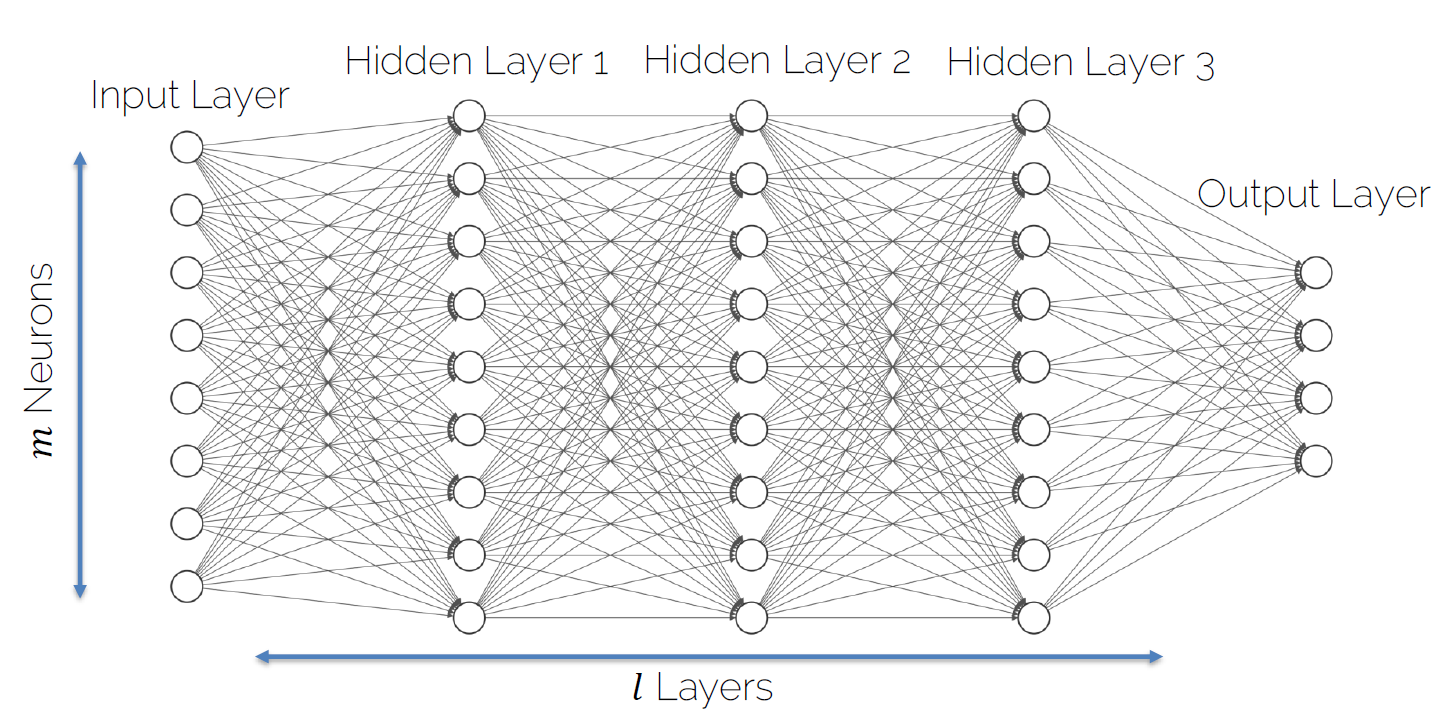
\includegraphics[width=\columnwidth]{figures/nn.png}
\end{figure} ~\\

\textbf{Mathematical Representation}
$$
	L = \mathcal L(y_j, \hat y_j, \theta)
$$
$$
	\hat y_j = a(s_{l,j})
$$
$$
	h_{i,j} = a(s_{i,j})
$$
$$
	s_{i,j} = b_{i,j} + \sum_{k = 1}^m h_{i-1,k} ⋅ w_{i,j,k}
$$
$$
	s_{1,j} = b_{1,j} + \sum_{k = 1}^m x_k ⋅ w_{1,j,k}
$$

\subsection{Number of weights}
\begin{tabular}{ll}	
	$l$: & Depth: number of layers \\
	$m_i$: & Width: number of neurons in layer $i$ (Here: layer $0$ is the input layer)\\
\end{tabular} ~\\

Number of weights is defined as:
$$
	\sum_{i = 1}^l m_i ⋅ m_{i-1} + m_i
$$

\subsection{Forward and Backward Pass}
\subsubsection{Forward Pass/ Forward Propagation}
Use formulas to calculate loss:
$$
	s_{1,1} = b_{1,1} + \sum_{k = 1}^m x_k ⋅ w_{1,1,k} \tab \dots \tab L = \mathcal L(y_j, \hat y_j)
$$

\subsection{Backward Pass/Backward Propagation}
\textbf{Weights of last layer:}
$$
	\frac{\partial L}{\partial w_{l,j,k}} = \frac{\partial L}{\partial \hat y_j} ⋅ \frac{\partial \hat y_j}{\partial s_{l,j}} ⋅ \frac{\partial s_{l,j}}{\partial w_{l,j,k}}
$$

\textbf{Weights of second last layer:}
$$
	\frac{\partial L}{\partial w_{l-1,j,k}} = \sum_{o = 1}^m \frac{\partial L}{\partial \hat y_o} ⋅ \frac{\partial \hat y_o}{\partial s_{l,o}} ⋅ \frac{\partial s_{l,o}}{\partial h_{l-1, j}} ⋅ \frac{\partial h_{l-1, j}}{\partial s_{l-1,j}} ⋅ \frac{\partial s_{l-1,j}}{\partial w_{l-1,j,k}}
$$

\textbf{General:}
$$
	\frac{\partial L}{\partial w_{i,j,k}} = \sum_{o_1 = 1}^m \dots \sum_{o_p = 1}^m \frac{\partial L}{\partial \hat y_{o_1}} ⋅ \frac{\partial \hat y_{o_1}}{\partial s_{l,o_1}} ~~⋅~~ \frac{\partial s_{l,o_1}}{\partial h_{l-1, o_2}} ⋅ \frac{\partial h_{l-1, o_2}}{\partial s_{l-1,o_2}} ⋅ \dots ⋅ \frac{\partial s_{i+1,o_p}}{\partial h_{i, j}} ⋅\frac{\partial h_{i, j}}{\partial s_{i,j}} ⋅ \frac{\partial s_{i,j}}{\partial w_{i,j,k}}
$$









\pagebreak
\section*{Notes}
This is a summary of the lecture~\lecture~of the Technical University Munich.
This lecture was presented by~\lecturer~in the~\semseter.
This summary was created by Gaida B.
All provided information is without guarantee.


%\section*{References}
%author. \textit{title}. publisher. location, year, 

\end{document}

%TODO check for todos








